\documentclass{article}
\usepackage{booktabs}   
\usepackage{geometry}
\usepackage{amsmath}
\usepackage{graphicx}
\usepackage{subcaption}
\geometry{margin=1in}

\title{Overview of presentation plots}
\author{Philipp Cremer, Jannis Stagge, Felix Westerhoff}

\begin{document}
\maketitle

\section{Replication}
\noindent \underline{Current OECD data}

\begin{figure}[htbp]
    \centering
    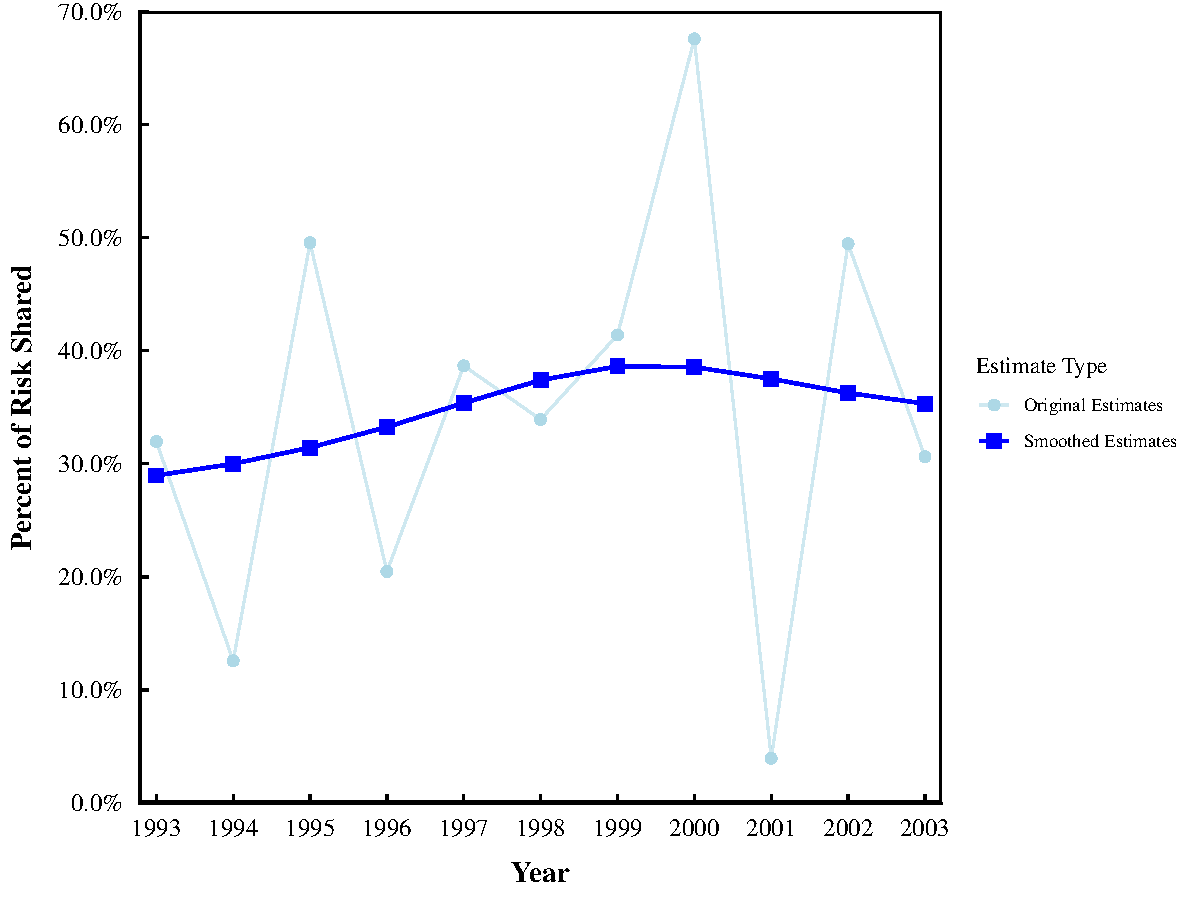
\includegraphics[width=\textwidth]{../output/rs_cs_rep_c.pdf}
    \caption{Replication of Consumption Risk Sharing}
\end{figure}

\begin{figure}[htbp]
        \centering
        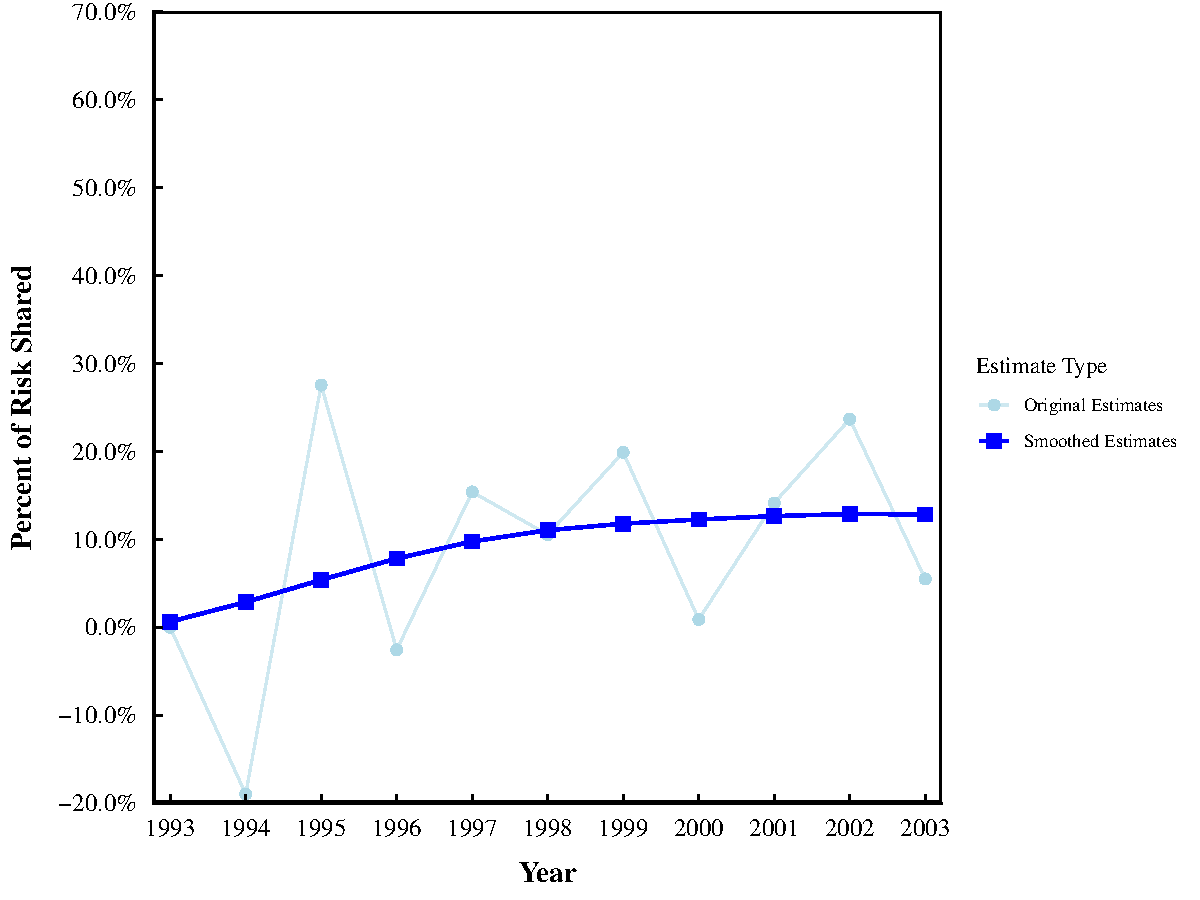
\includegraphics[width=\textwidth]{../output/rs_cs_rep_i.pdf}
        \caption{Replication of Income Risk Sharing}
\end{figure}

\newpage

\noindent \underline{Past OECD data ("Sanity Check")}
\begin{figure}[htbp]
    \centering
    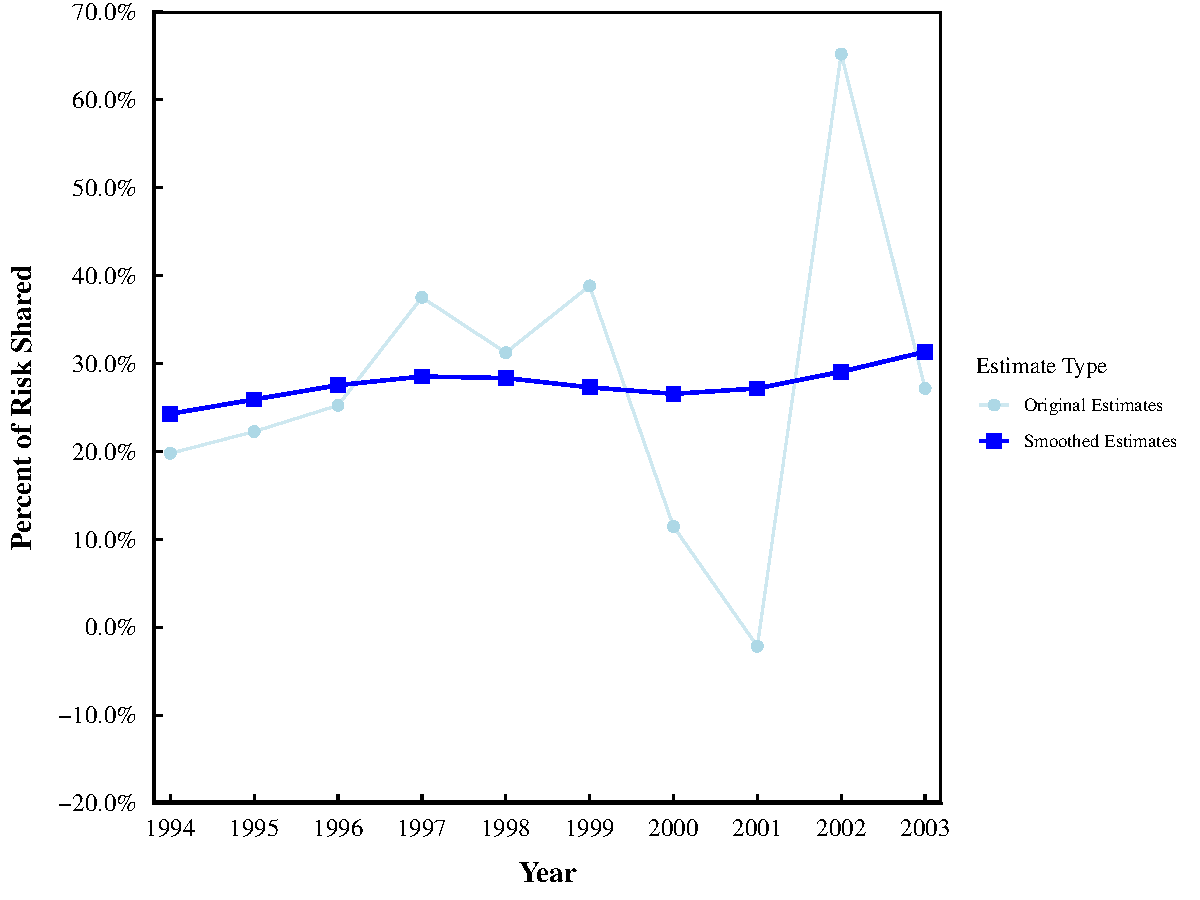
\includegraphics[width=\textwidth]{../output/rs_cs_sanity_c.pdf}
    \caption{(Extracted) consumption risk sharing, 2005 constant prices, no government exp.}
\end{figure}

\begin{figure}[htbp]
    \centering
    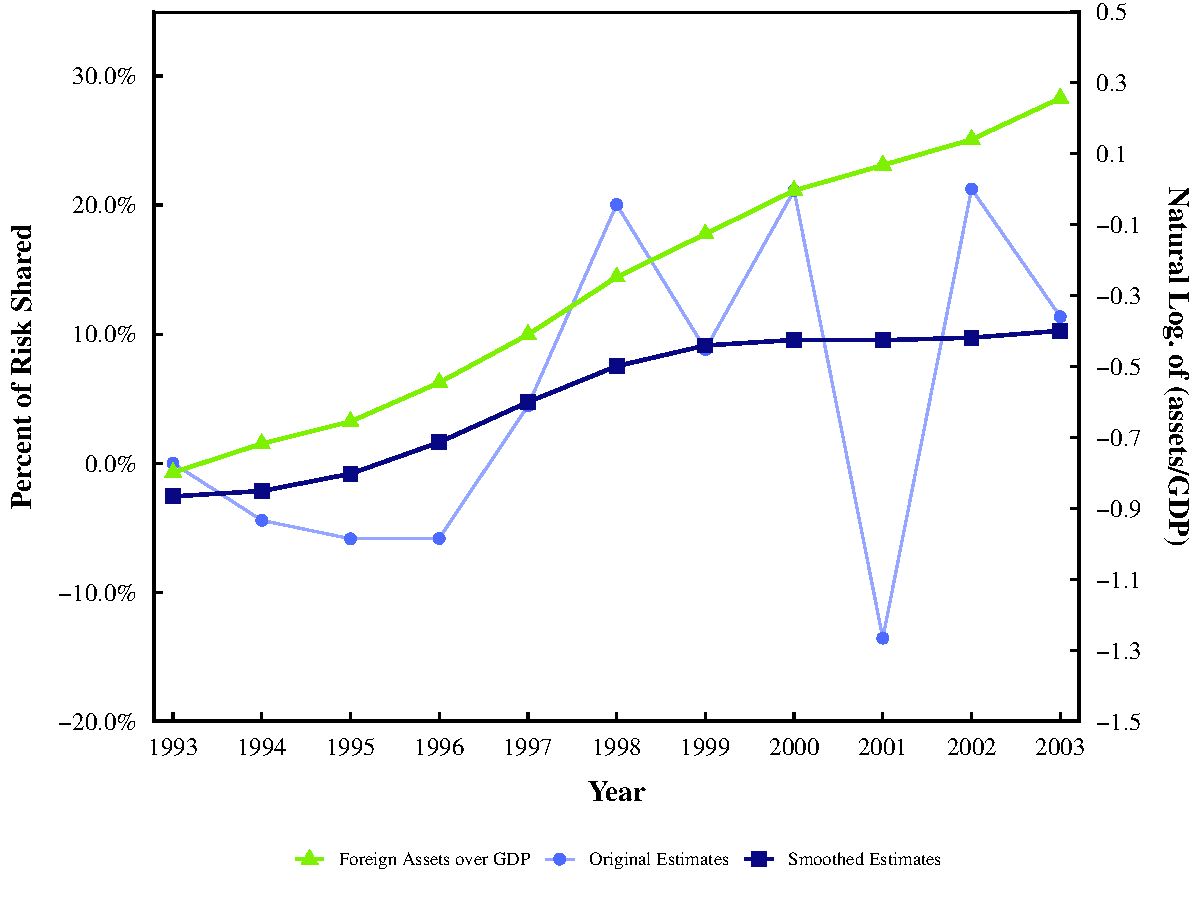
\includegraphics[width=\textwidth]{../output/rs_cs_sanity_i.pdf}
    \caption{Manually computed PPP adjustment from extracted data}
\end{figure}

\newpage

\section{Extensions}
\noindent \underline{Extension 1: 1987 - 2017, same countries}

\begin{figure}[htbp]
    \centering
    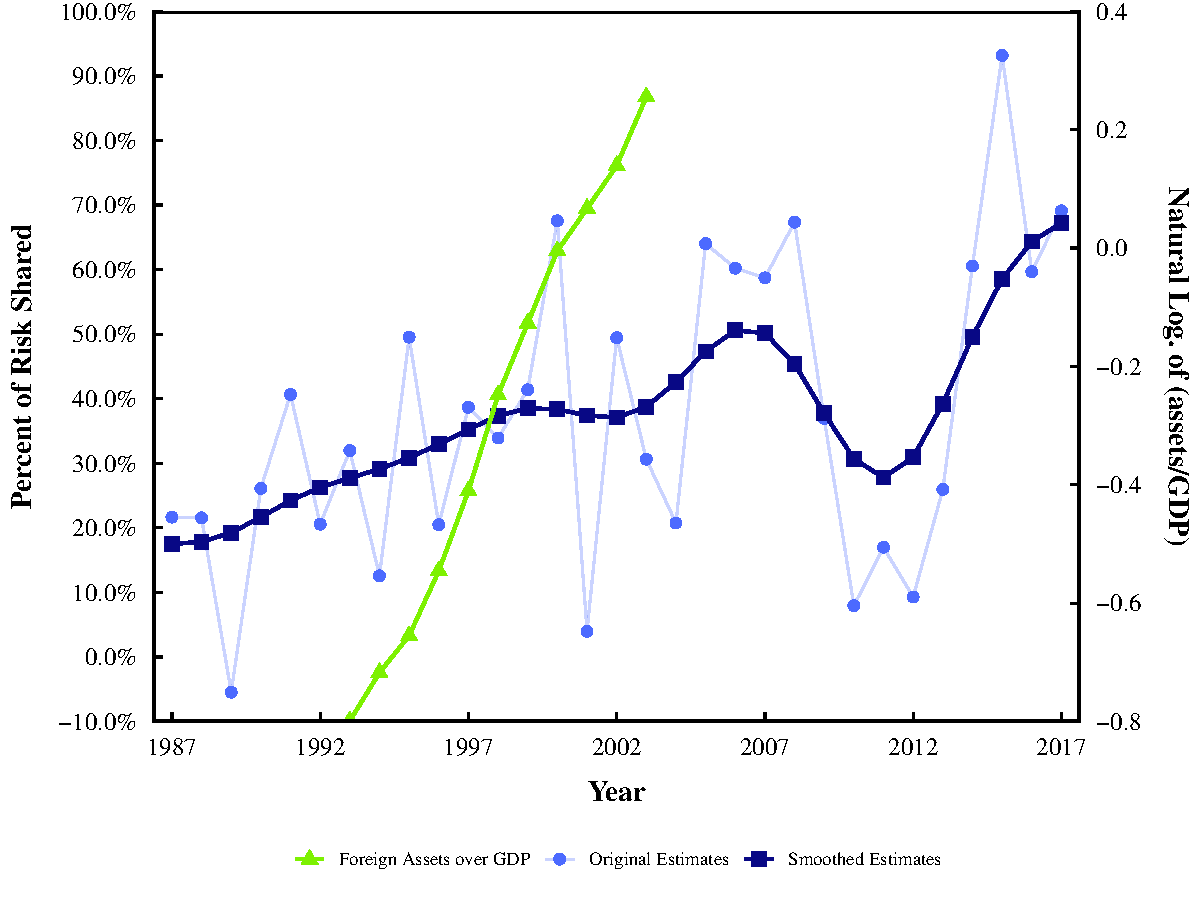
\includegraphics[width=\textwidth]{../output/rs_cs_ext_1_c.pdf}
    \caption{Consumption Risk Sharing}
\end{figure}

\begin{figure}[htbp]
        \centering
        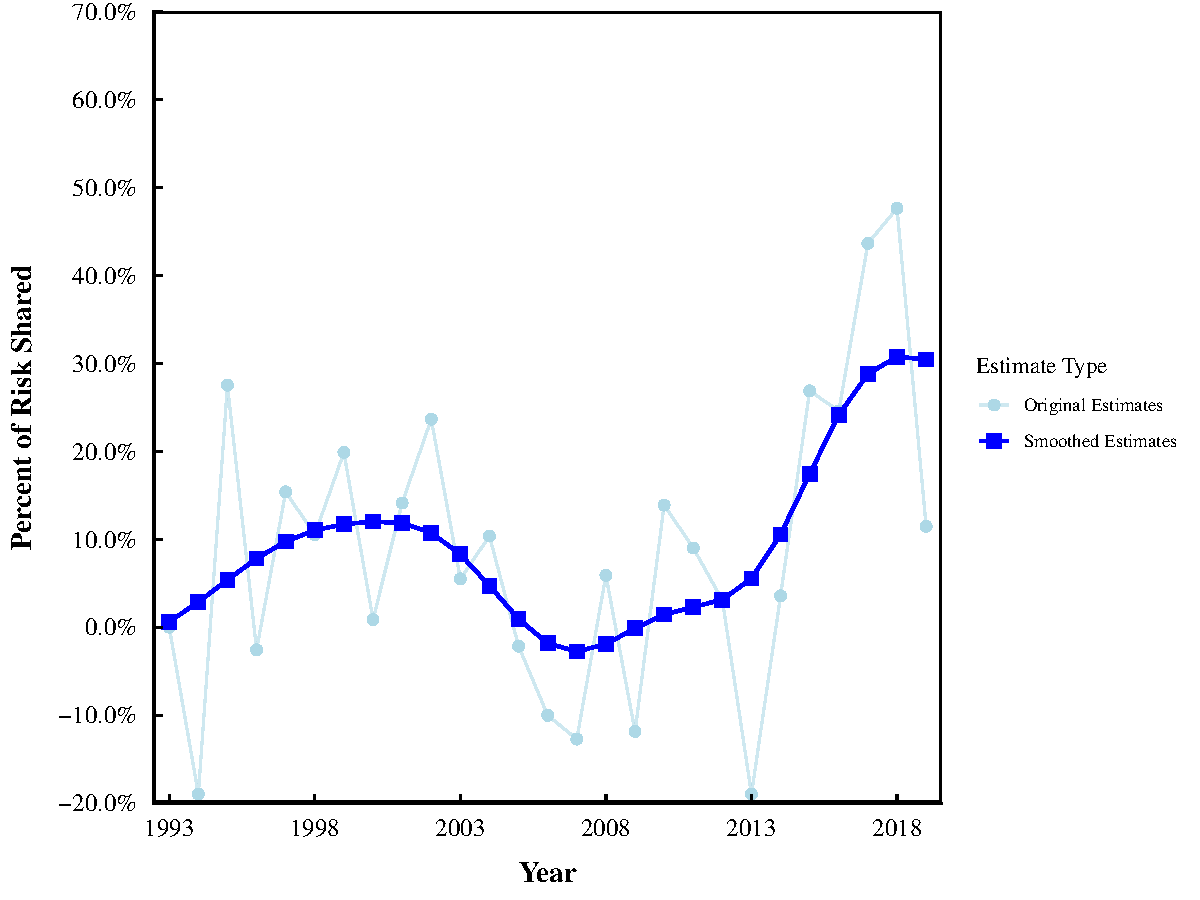
\includegraphics[width=\textwidth]{../output/rs_cs_ext_1_i.pdf}
        \caption{Income Risk Sharing}
\end{figure}

\newpage

\noindent \underline{Extension 2: 1987 - 2017, Top 50 Economies + EU (depending on data availability)}

\begin{figure}[htbp]
    \centering
    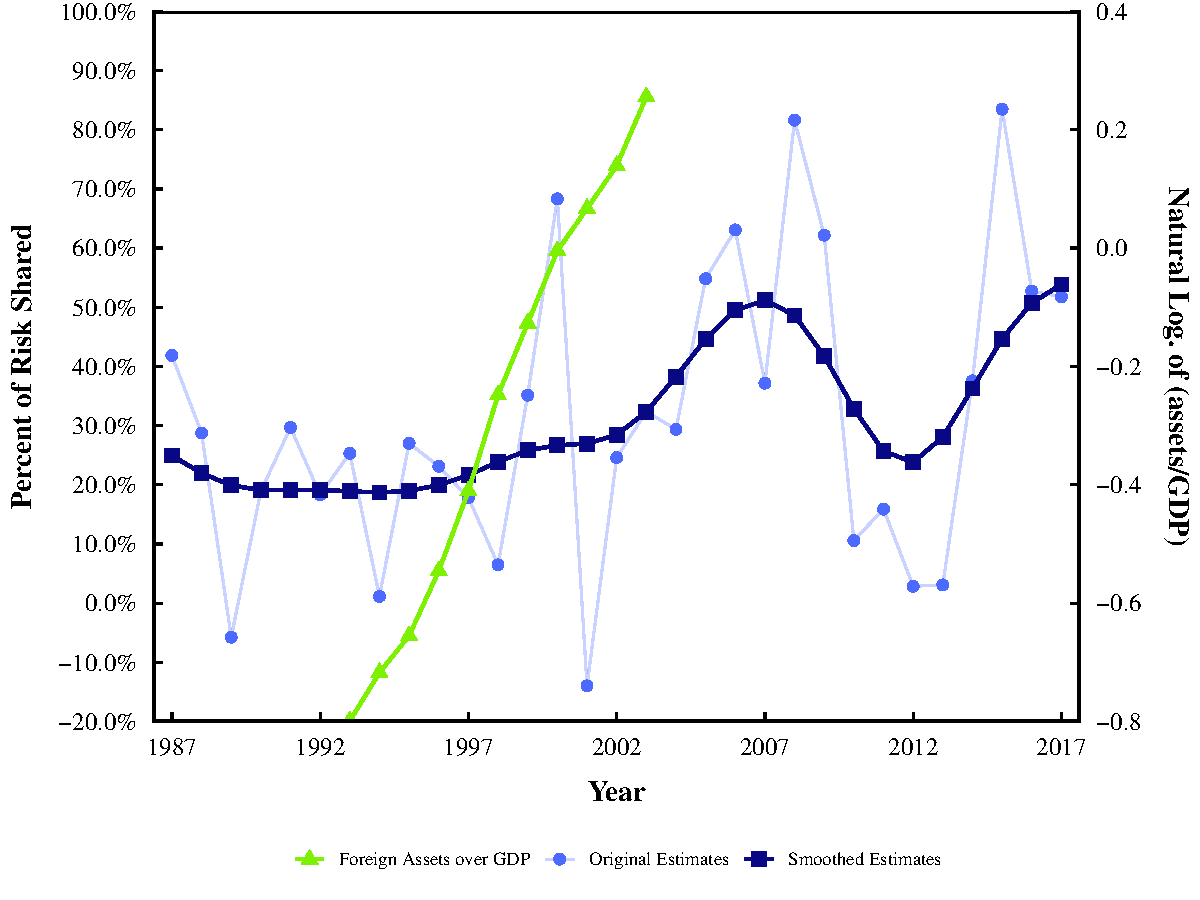
\includegraphics[width=\textwidth]{../output/rs_cs_ext_2_c.pdf}
    \caption{Consumption Risk Sharing}
\end{figure}

\begin{figure}[htbp]
        \centering
        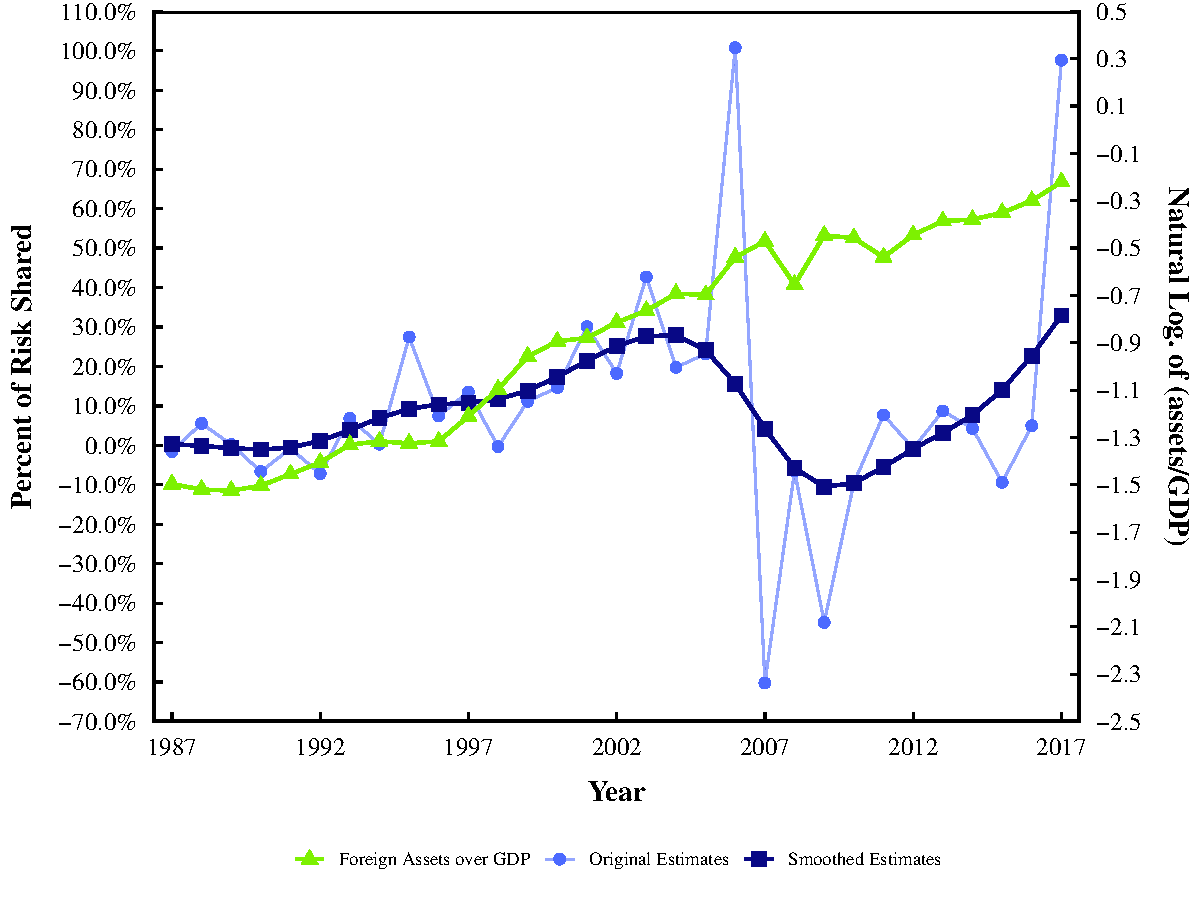
\includegraphics[width=\textwidth]{../output/rs_cs_ext_2_i.pdf}
        \caption{Income Risk Sharing}
\end{figure}

\newpage

\noindent \underline{Extension 3: 1987 - 2017, Eurozone}

\begin{figure}[htbp]
    \centering
    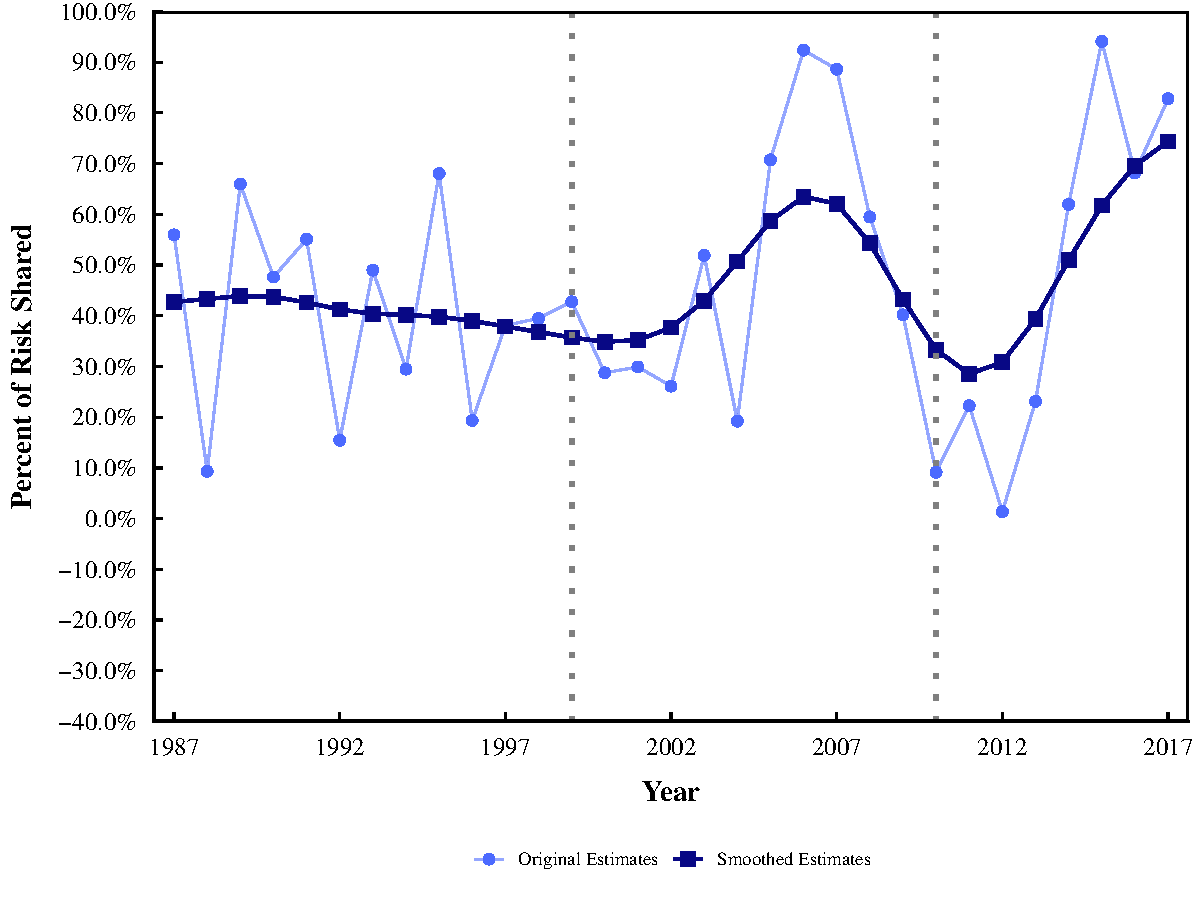
\includegraphics[width=\textwidth]{../output/rs_cs_ext_3_c.pdf}
    \caption{Consumption Risk Sharing}
\end{figure}

\begin{figure}[htbp]
        \centering
        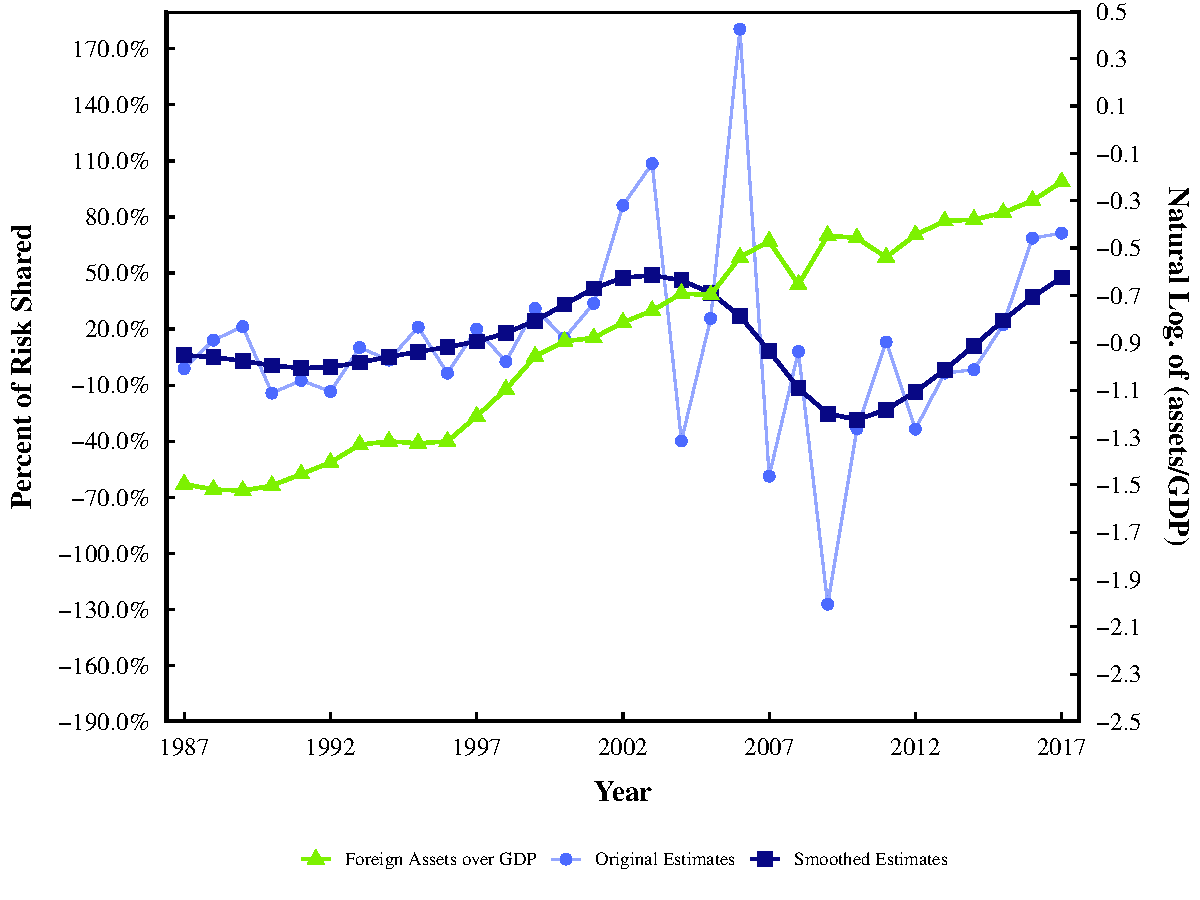
\includegraphics[width=\textwidth]{../output/rs_cs_ext_3_i.pdf}
        \caption{Income Risk Sharing}
\end{figure}

\newpage

\section{Channels of Risk Sharing}
\begin{figure}[htbp]
    \centering
    
    % First subfigure
    \begin{subfigure}[b]{0.32\textwidth}
        \centering
        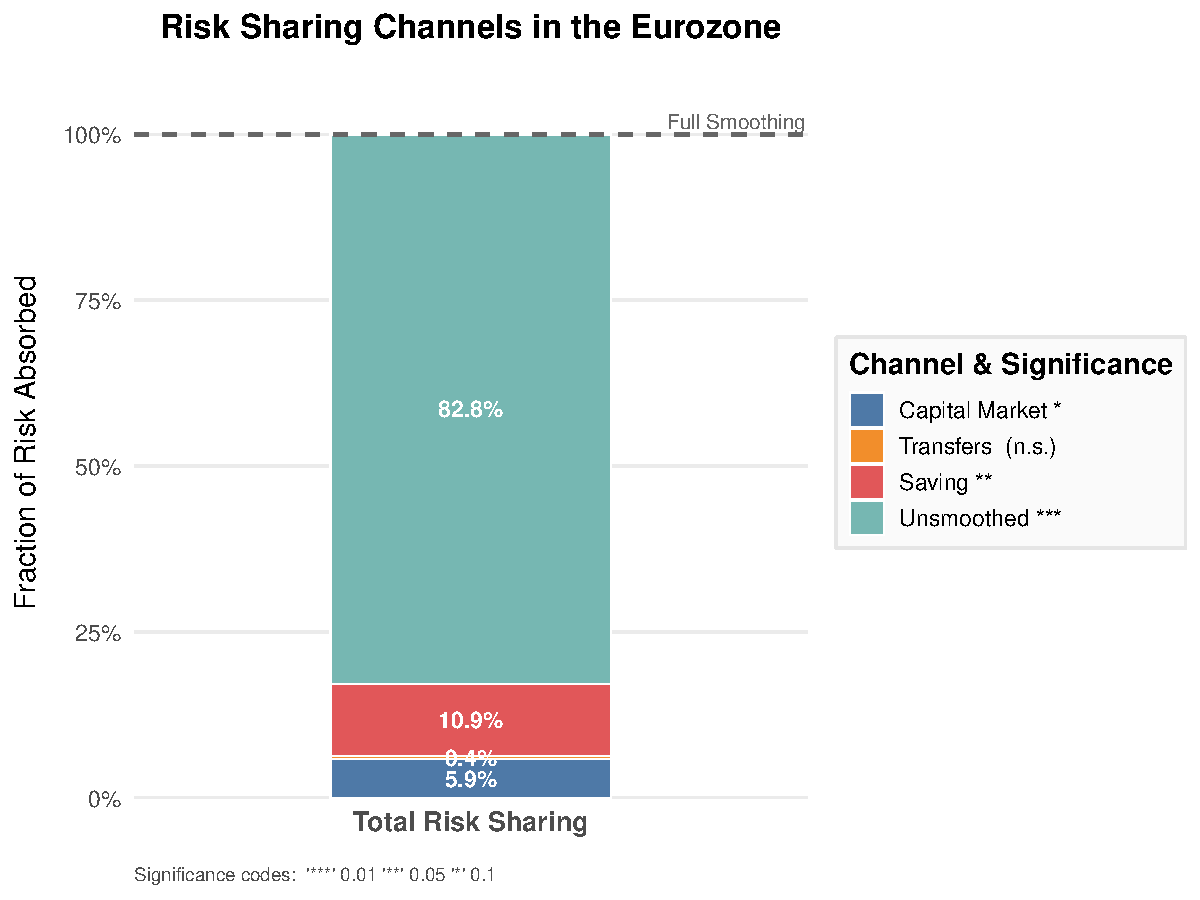
\includegraphics[width=\textwidth]{../output/ea_95_23.pdf}
        \caption{1995 -- 2023}
    \end{subfigure}
    \hfill
    % Second subfigure
    \begin{subfigure}[b]{0.32\textwidth}
        \centering
        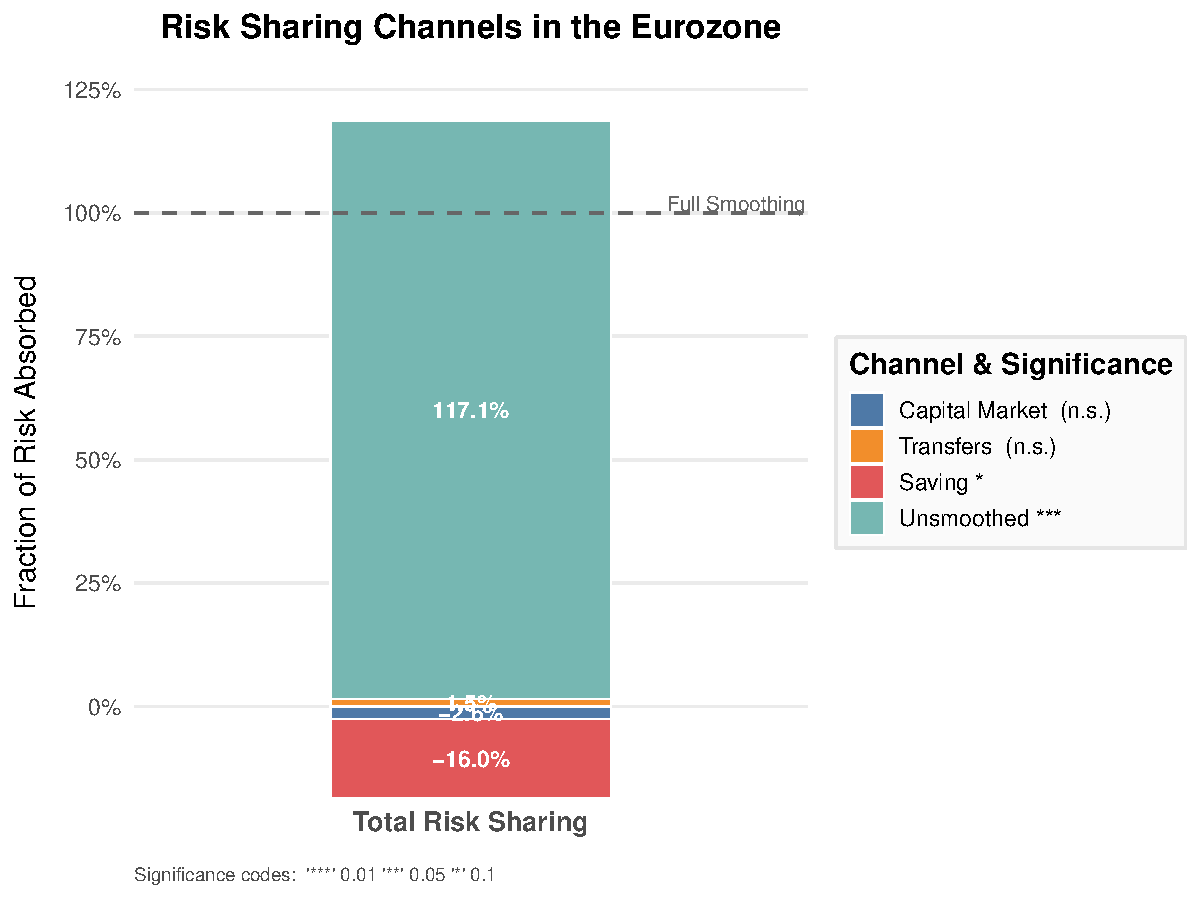
\includegraphics[width=\textwidth]{../output/ea_95_07.pdf}
        \caption{1995 -- 2007}
    \end{subfigure}
    \hfill
    % Third subfigure
    \begin{subfigure}[b]{0.32\textwidth}
        \centering
        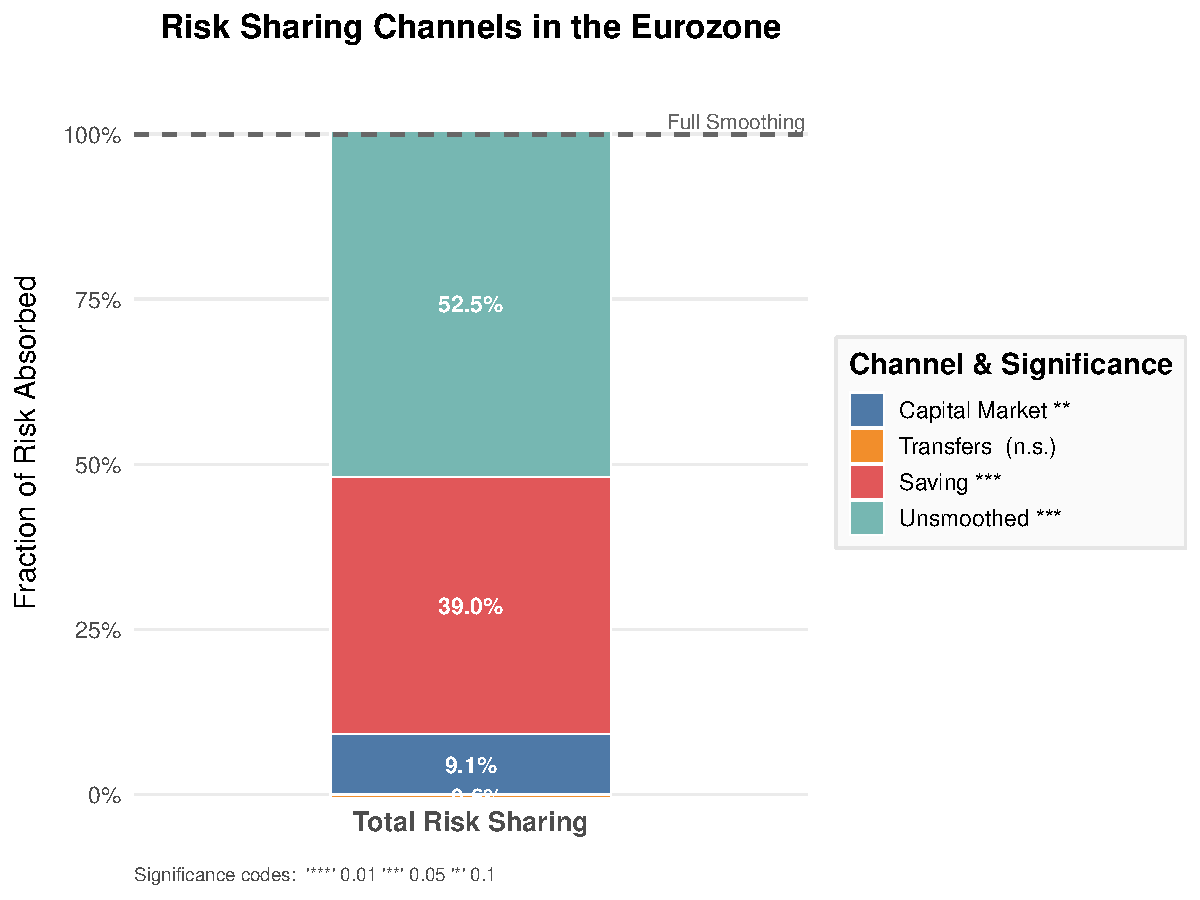
\includegraphics[width=\textwidth]{../output/ea_10_23.pdf}
        \caption{2010 -- 2023}
    \end{subfigure}
    
    \caption{Risk Sharing Channels in the Eurozone: Different time periods (Panel Estimation)}
\end{figure}

\begin{figure}[htbp]
        \centering
        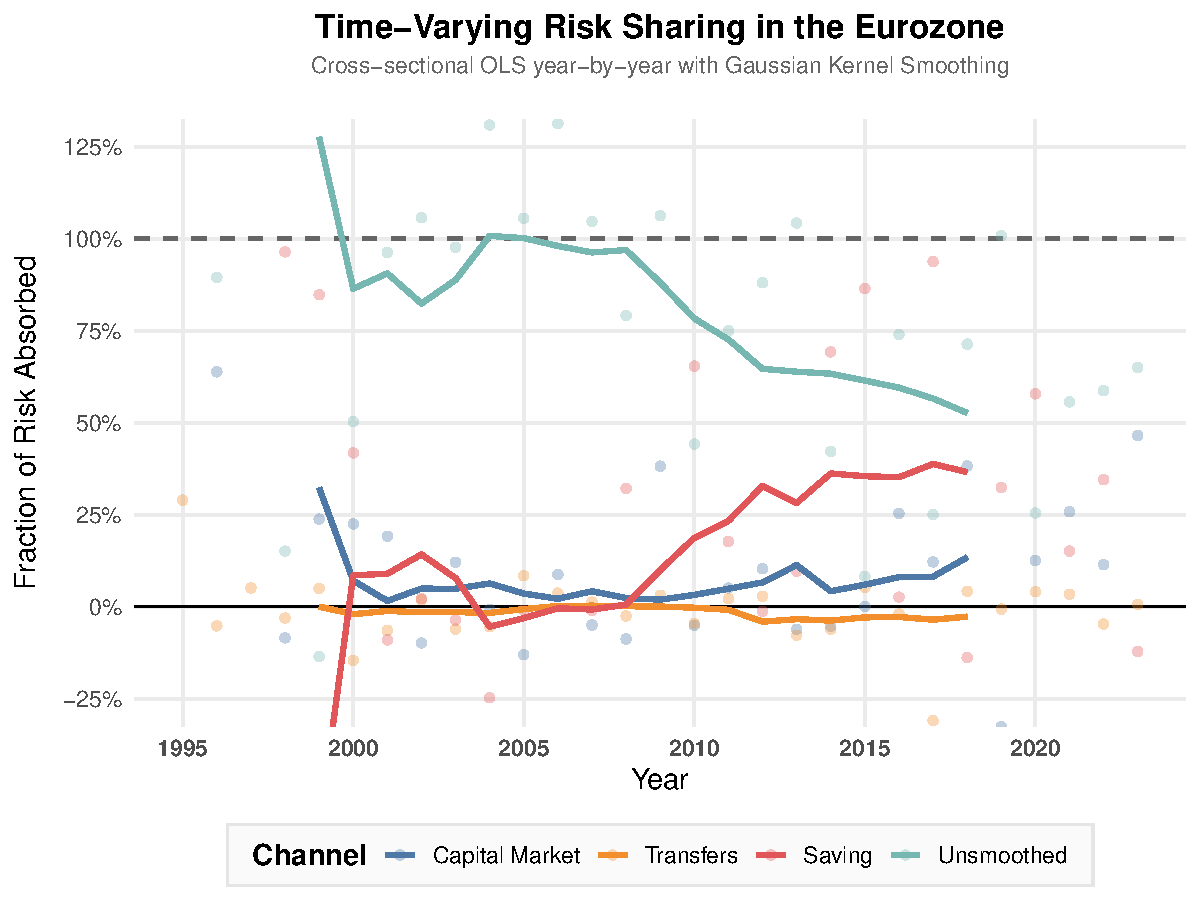
\includegraphics[width=\textwidth]{../output/channels_cross_section.pdf}
        \caption{Risk Sharing Channels in the Eurozone: Year-by-year cross-sectional estimates (10-year centred moving averages)}
\end{figure}

\end{document}
